\subsection{Unser and Beam Current Monitors Calibration}
In order to accurately calibrate the BCM's, first the unser must be calibrated. The unser is used as an absolute reference to which the BCM's are calibrated to. The procedure to calibrate the unser involves sending a constant and known currents through a thin wire inside of the unser. A series of currents with, over a range between 2.5 - 100 $\mu$A,during 90 second intervals, as can be seen in figure (??). which shows the frequency response of the unser for the various currents. A linear fit of sent current vs the unser response, determines an overall gain factor for the unser. The gain of the unser of calibrated 4 times during MARATHON before each BCM calibration was preformed, in order to check the unser's stability. Figure(??) shows the unser was stable during the entirety of the MARATHON run. 

\begin{table}[ht]
\caption{Unser Calibration Results}
%\centering
\begin{center}
\begin{tabular}{l| c| c| c| r}
Date & 03-05 & 03-28 & 4-03 & 04-06  \\
\hline
Unser Gain & 2.526e-4 & 2.524e-4 & 2.529e-4 & 2.527e-4\\
\end{tabular}
\end{center}
\end{table}

Having calibrated the unser, we can then calibrate the BCMs in a similar manner to the calibration of the unser but replacing the current from a wire with current from the electron beam. For the BCM calibrations during MARATHON and all Tritium experiments, the range in current was between 3 - 22.5 $\mu$A. Again, the procedure intervals of 90 seconds (i.e 90 seconds of continuous current to the Hall followed by 90 seconds with no beam). 
The Calibration procedure requires making cuts in the frequency response of the unser and BCM receiver and integrating the total amount of frequency to determine the average frequency of the receiver during the given time interval. An example of the cuts made is shown in figure 3

The unser frequency during the calibration can be related to the delivered current using the gain factor determined from the unser calibration. 
\begin{equation}
I_{unser} = gain * f_{unser}
\end{equation}

By then plotting $I_{unser} vs freq_{BCM}$ and fitting with a linear function, the gain and offset (which are proportional the slope and intercept of the fit respectively) of each BCM receiver can be determined. The gain 



%unser
\begin{figure}[H]
\begin{center}
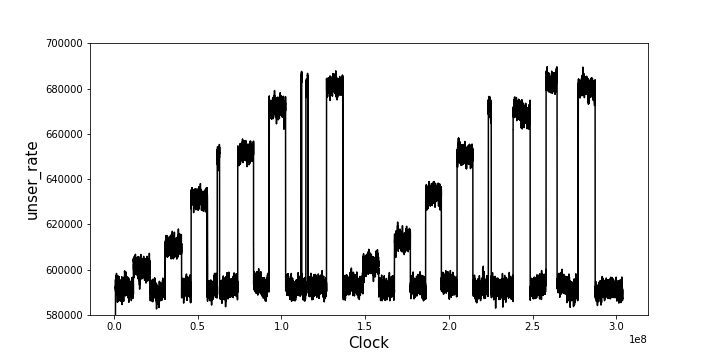
\includegraphics[angle=0, scale =0.65]{Unser_freq.png}
\end{center}
\caption{BCM Calibration : unser}
\end{figure}
%dnew
\begin{figure}[H]
\begin{center}
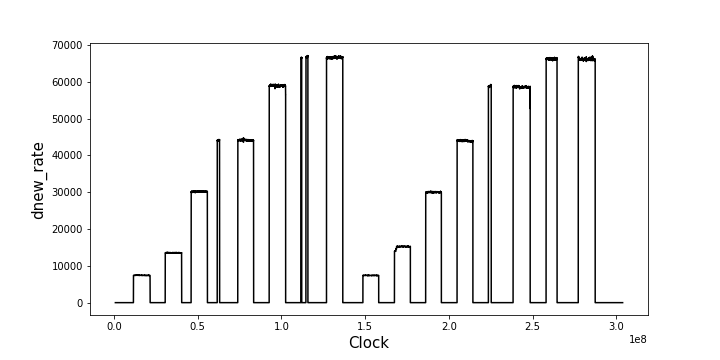
\includegraphics[angle=0, scale =0.65]{Dnew_freq.png}
\end{center}
\caption{BCM Calibration : dnew}
\end{figure}


\begin{figure}[H]
\begin{center}
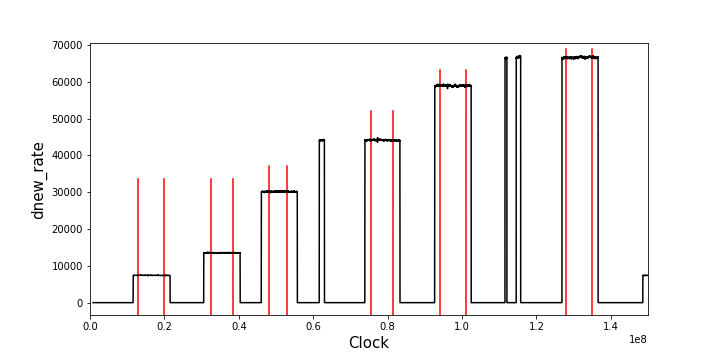
\includegraphics[angle=0, scale =0.65]{Dnew_freq_cuts.png}
\end{center}
\caption{Frequency cuts}
\end{figure}

Table(??) shows the result of the 3 BCM calibrations for the dnew digital BCM receiver.
\begin{table}[ht]
\caption{BCM Calibration Results}
%\centering
\begin{center}
\begin{tabular}{l| c| c| r}
   & 03-05 & 03-28 & 4-03 \\
\hline
dnew Gain & 3.3358e-4 & 3.3351e-4 & 3.3372e-4\\
\hline
dnew offset & -0.097  &   0.003   & 0.132         \\
\end{tabular}
\end{center}
\end{table}
